\documentclass[aspectratio=169, 12pt]{beamer}

\usetheme{Madrid}
\usecolortheme{seahorse}

\usepackage{graphicx}
\usepackage{booktabs}
\usepackage{hyperref}
\usepackage{xcolor}
\usepackage{tikz}

\graphicspath{{plot_guide_screenshots/}}

% --- Light, high-contrast theme ---
\definecolor{SlideBg}{HTML}{F7FAFC}
\definecolor{SlideText}{HTML}{18212F}
\definecolor{SlideMuted}{HTML}{64748B}
\definecolor{AccentBlue}{HTML}{1D4ED8}
\definecolor{AccentPanel}{HTML}{DBEAFE}
\definecolor{FrameBar}{HTML}{E2E8F0}
\definecolor{BlockFill}{HTML}{EEF6FF}

\setbeamercolor{background canvas}{bg=SlideBg}
\setbeamercolor{normal text}{fg=SlideText}
\setbeamercolor{frametitle}{fg=SlideText, bg=FrameBar}
\setbeamercolor{title}{fg=SlideText, bg=AccentPanel}
\setbeamercolor{subtitle}{fg=SlideMuted}
\setbeamercolor{author}{fg=SlideText}
\setbeamercolor{date}{fg=SlideMuted}
\setbeamercolor{institute}{fg=SlideMuted}
\setbeamercolor{item}{fg=AccentBlue}
\setbeamercolor{block title}{fg=white, bg=AccentBlue}
\setbeamercolor{block body}{fg=SlideText, bg=BlockFill}
\setbeamercolor{structure}{fg=AccentBlue}
\setbeamercolor{alerted text}{fg=AccentBlue}

\setbeamertemplate{navigation symbols}{}
\setbeamertemplate{footline}{%
  \begin{tikzpicture}[remember picture,overlay]
    \node[anchor=south east,text=SlideMuted,font=\scriptsize]
      at ([xshift=-0.25cm,yshift=0.12cm]current page.south east)
      {\insertframenumber/\inserttotalframenumber};
  \end{tikzpicture}%
}

\title{Communications Systems Visualizer}
\subtitle{ENGR 78 Final Project \textemdash\ Interactive browser dashboard (Dash/Plotly)}
\author[Wang, Moo, Schuetz]{Howard Wang \and Kaw Moo \and Charlie Schuetz}
\institute{ENGR 78 \textbullet\ Spring 2026}

\begin{document}

% --- Title ---
\begin{frame}[plain]
\vspace{0.95cm}
\begin{center}
\begin{beamercolorbox}[wd=0.88\linewidth,sep=0.38cm,center,rounded=true,shadow=false]{title}
{\LARGE\bfseries Communications Systems Visualizer}\\[0.3cm]
{\normalsize ENGR 78 Final Project}
\end{beamercolorbox}
\vspace{0.75cm}
{\large Howard Wang \quad Kaw Moo \quad Charlie Schuetz}\\[0.45cm]
{\normalsize\color{SlideMuted}Spring 2026}
\end{center}
\end{frame}

% --- Motivation ---
\begin{frame}{Motivation}
\begin{itemize}
    \item ENGR~78 spans sampling, baseband signaling, pulse design, passband modulation, and information limits---often taught as \textbf{separate} problem sets or static plots.
    \item Students benefit from \alert{one place} where sliders and inputs change \textbf{linked} time-domain, frequency-domain, and statistical views at once.
    \item A locally hosted \textbf{Dash} app keeps the demo reproducible in any classroom or dorm room without bench hardware.
\end{itemize}
\end{frame}

% --- Objective ---
\begin{frame}{Project objective}
\begin{enumerate}
    \item Build a \textbf{browser-based ENGR~78 learning visualizer}, not a hardware-dependent SDR lab.
    \item Let users adjust course parameters---bits, bandwidth, roll-off, noise, symbol rate, and modulation order---and see \textbf{linked} waveforms, spectra, eye/constellation views, throughput, and capacity results.
    \item Keep the core demo \textbf{laptop-only} with \texttt{python main.py}; treat \textbf{ADALM-PLUTO} live mode as a separate optional extension.
\end{enumerate}
\end{frame}

% --- Overview ---
\begin{frame}{Overview: how the app works}
\small
\begin{center}
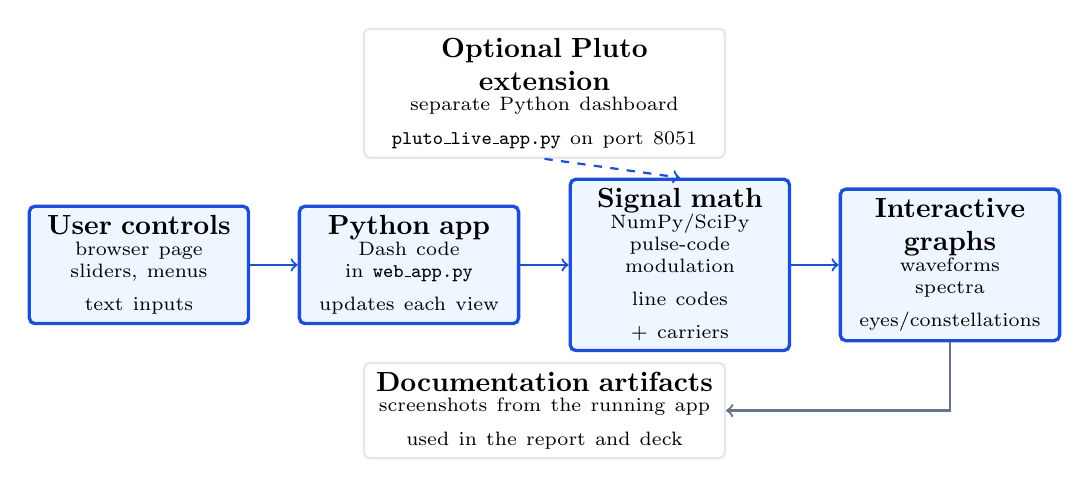
\begin{tikzpicture}[
    appbox/.style={draw=AccentBlue, fill=BlockFill, rounded corners=2pt, very thick,
                   align=center, minimum height=1.35cm, text width=2.55cm},
    supportbox/.style={draw=FrameBar, fill=white, rounded corners=2pt, thick,
                       align=center, minimum height=0.95cm, text width=4.35cm},
    arrow/.style={->, thick, draw=AccentBlue}
]
    \node[appbox] (ui) at (-5.15,0)
        {\textbf{User controls}\\[-0.02cm]
        {\scriptsize browser page\\sliders, menus\\text inputs}};
    \node[appbox] (callbacks) at (-1.72,0)
        {\textbf{Python app}\\[-0.02cm]
        {\scriptsize Dash code\\in \texttt{web\_app.py}\\updates each view}};
    \node[appbox] (signals) at (1.72,0)
        {\textbf{Signal math}\\[-0.02cm]
        {\scriptsize NumPy/SciPy\\pulse-code modulation\\line codes + carriers}};
    \node[appbox] (plots) at (5.15,0)
        {\textbf{Interactive graphs}\\[-0.02cm]
        {\scriptsize waveforms\\spectra\\eyes/constellations}};

    \draw[arrow] (ui) -- (callbacks);
    \draw[arrow] (callbacks) -- (signals);
    \draw[arrow] (signals) -- (plots);

    \node[supportbox] (pluto) at (0,2.18)
        {\textbf{Optional Pluto extension}\\[-0.02cm]
        {\scriptsize separate Python dashboard\\\texttt{pluto\_live\_app.py} on port 8051}};
    \draw[arrow, dashed] (pluto.south) -- (signals.north);

    \node[supportbox] (docs) at (0,-1.85)
        {\textbf{Documentation artifacts}\\[-0.02cm]
        {\scriptsize screenshots from the running app\\used in the report and deck}};
    \draw[->, thick, draw=SlideMuted] (plots.south) |- (docs.east);
\end{tikzpicture}
\end{center}
\vspace{-0.08cm}
{\scriptsize\color{SlideMuted}Core path: user changes a control $\rightarrow$ Python recomputes the signal data $\rightarrow$ Plotly redraws the graphs.\par}
\end{frame}

% --- Screenshot 1 ---
\begin{frame}{Dashboard (carrier tab: QPSK)}
\vspace{-0.2cm}
\begin{center}
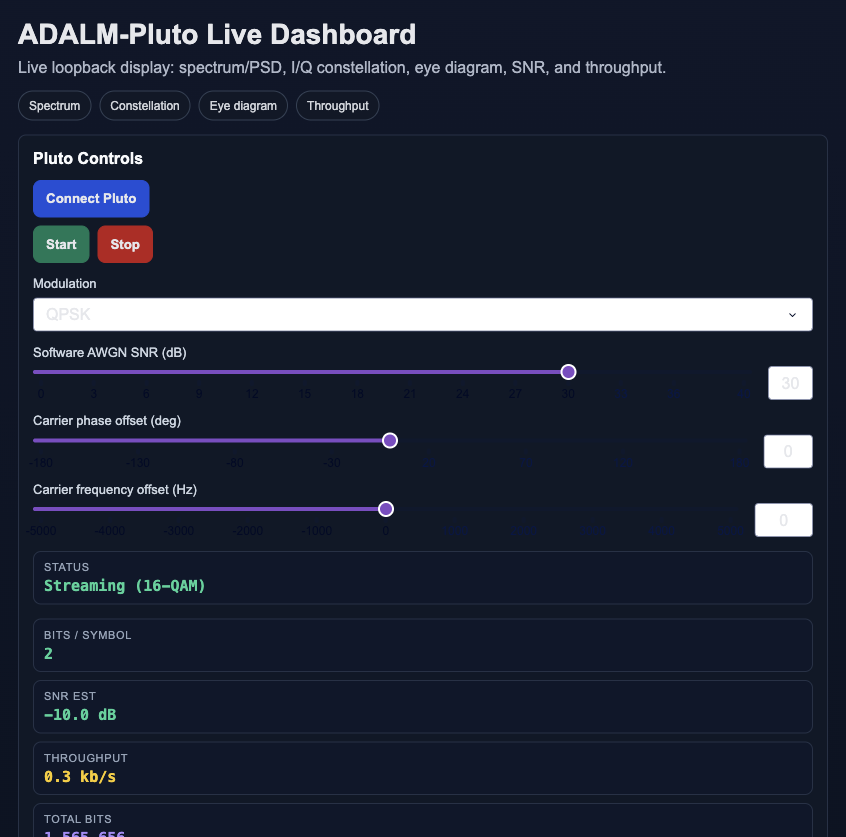
\includegraphics[width=0.98\linewidth,height=0.72\textheight,keepaspectratio]{dashboard_visible_qpsk.png}
\end{center}
\vspace{-0.12cm}
{\scriptsize\color{SlideMuted}Tab navigation, summary statistics, and synchronized Plotly panels.}
\end{frame}

% --- Screenshot 2 ---
\begin{frame}{Composite plot export}
\vspace{-0.15cm}
\begin{center}
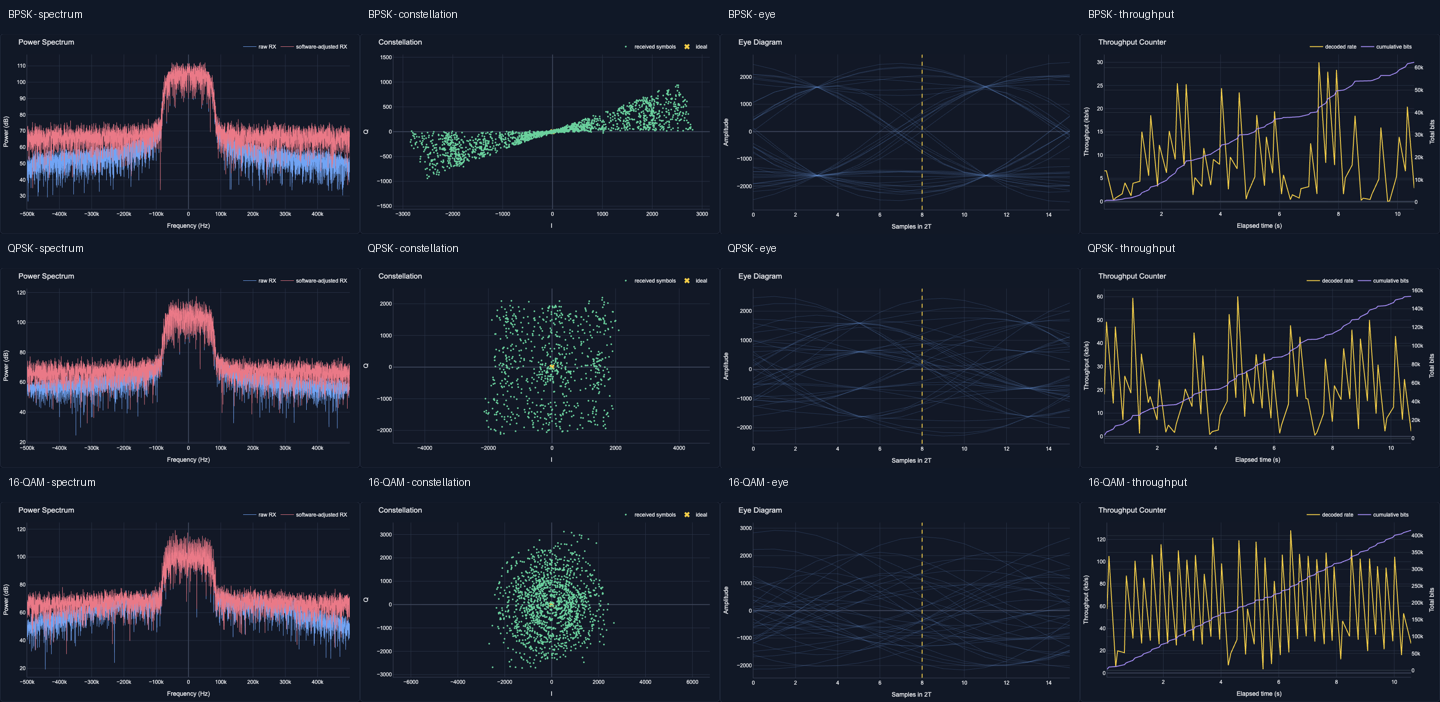
\includegraphics[width=0.98\linewidth,height=0.72\textheight,keepaspectratio]{plot_contact_sheet.png}
\end{center}
\vspace{-0.1cm}
{\scriptsize\color{SlideMuted}Single image combining constellation, spectrum, eye, and throughput views for documentation.}
\end{frame}

% --- Screenshot 3 ---
\begin{frame}{Full-dashboard capture (BPSK)}
\vspace{-0.2cm}
\begin{center}
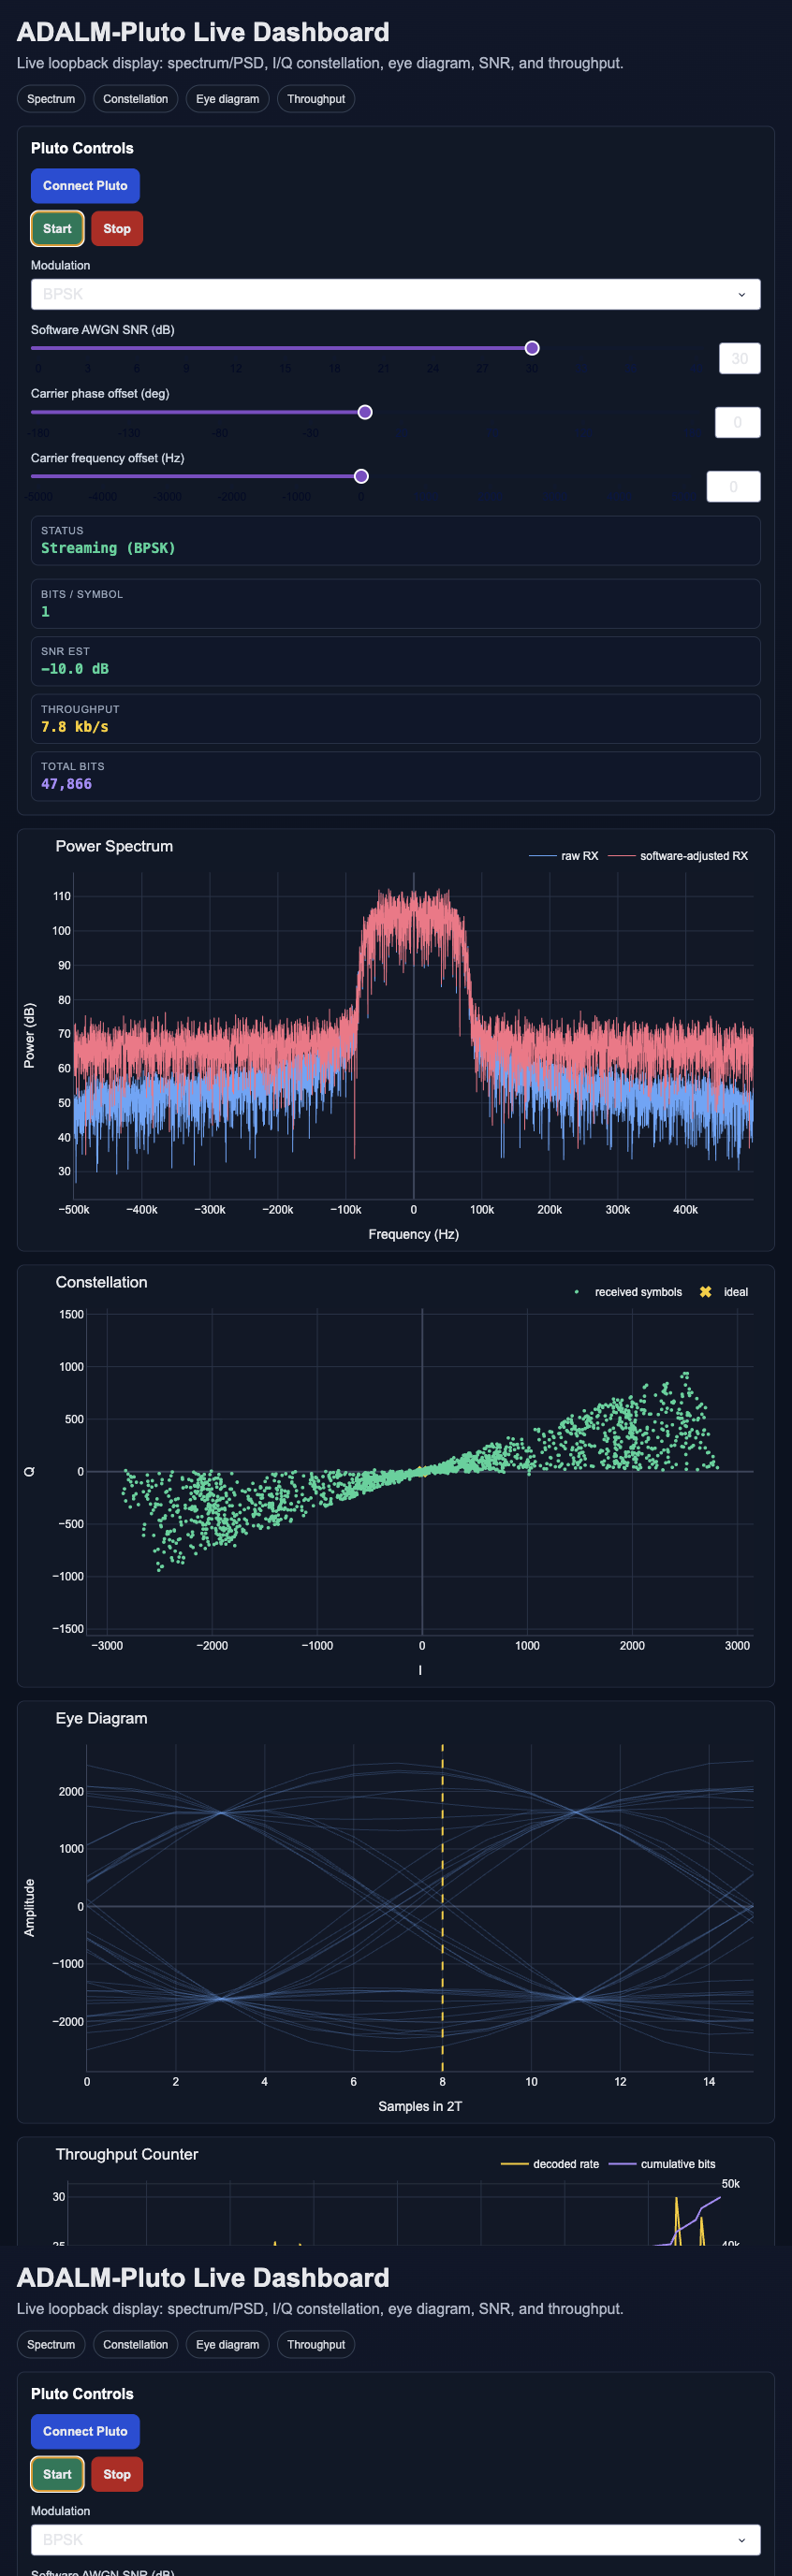
\includegraphics[width=0.95\linewidth,height=0.72\textheight,keepaspectratio]{bpsk_full.png}
\end{center}
\end{frame}

% --- Screenshot 4 ---
\begin{frame}{Constellation and eye diagram (QPSK)}
\begin{columns}[c,onlytextwidth]
\begin{column}{0.49\linewidth}
\centering
\begin{tikzpicture}
    \node[draw=AccentBlue, line width=1.7pt, rounded corners=3pt, inner sep=2pt] (img)
        {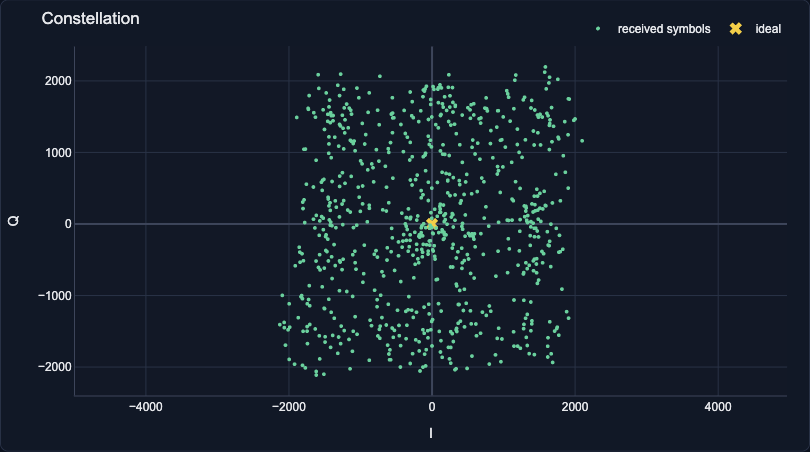
\includegraphics[width=0.95\linewidth,height=0.53\textheight,keepaspectratio]{qpsk_constellation.png}};
    \node[anchor=north west, fill=AccentBlue, text=white, rounded corners=2pt,
          font=\scriptsize\bfseries, inner xsep=4pt, inner ysep=2pt]
        at ([xshift=0.08cm,yshift=-0.08cm]img.north west) {Extra visualization};
\end{tikzpicture}\\[0.08cm]
{\scriptsize\color{AccentBlue}\textbf{Constellation: symbol map}}
\end{column}
\begin{column}{0.49\linewidth}
\centering
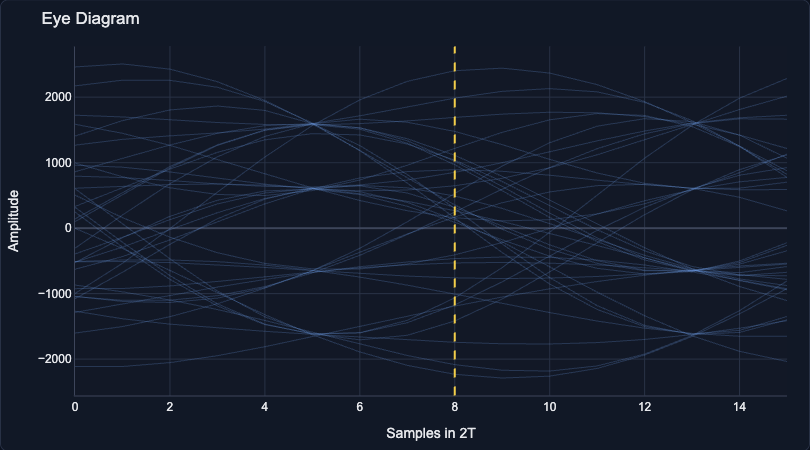
\includegraphics[width=\linewidth,height=0.55\textheight,keepaspectratio]{qpsk_eye.png}\\[0.1cm]
{\scriptsize Eye diagram}
\end{column}
\end{columns}
\end{frame}

% --- Feature detail ---
\begin{frame}{Tabs I\textemdash III: baseband and channel}
\small
\begin{itemize}
    \item \textbf{PCM} --- bandwidth $B_m$, oversampling vs.\ Nyquist, bits per sample $n$, implied PCM bit rate and waveform sketch.
    \item \textbf{Line coding} --- user bit string (up to 32 bits), NRZ/RZ on-off and polar, AMI, Manchester; waveform + windowed PSD.
    \item \textbf{ISI + eye} --- raised-cosine roll-off $\beta$, neighbor-symbol coupling, Gaussian noise, PAM order; overlaid eye segments after matched filtering.
\end{itemize}
\end{frame}

% --- Feature detail 2 ---
\begin{frame}{Tabs IV\textemdash V: passband and information}
\small
\begin{itemize}
    \item \textbf{$M$-ary + carrier} --- PAM spacing, symbol rate $R_s$, ASK/OOK, BPSK, BFSK, QPSK, 16-QAM time/spectrum views; throughput and cumulative bits.
    \item \textbf{Capacity + codes} --- Shannon $C=B\log_2(1+\mathrm{SNR})$ vs.\ SNR with operating point; discrete source entropy; repetition-code Hamming-distance toy.
\end{itemize}
\vfill
{\small\color{SlideMuted}\textbf{Implementation:} Core logic and callbacks live in \texttt{web\_app.py}; \texttt{main.py} only starts the server.\par}
\end{frame}

% --- Optional Pluto ---
\begin{frame}{Optional hardware path}
\begin{itemize}
    \item \texttt{pluto\_live\_app.py}: second Dash app (default \textbf{port 8051}) streaming IQ through \texttt{RealtimeEngine} (\texttt{src/realtime\_engine.py}). Use \textbf{Simulation (no radio)} without hardware, then \textbf{Start}.
    \item Typical schemes in the live UI: BPSK, QPSK, 16-QAM; spectrum, constellation, eye, SNR/throughput trends.
    \item macOS: Pluto USB Ethernet in \texttt{ncm} mode; device often at \texttt{192.168.2.1} (see repository \texttt{README.md}).
\end{itemize}
\vfill
{\small\color{SlideMuted}Course grading and demos can rely entirely on the browser app; Pluto is additive.\par}
\end{frame}

% --- File roles (compact) ---
\begin{frame}{Key files}
\centering
\footnotesize
\begin{tabular}{@{}ll@{}}
\toprule
\textbf{File} & \textbf{Role} \\
\midrule
\texttt{main.py} & Entry point; runs Dash on localhost (port 8050). \\
\texttt{web\_app.py} & Tabs, callbacks, NumPy/Plotly signal generation \\
\texttt{pluto\_live\_app.py} & Optional Pluto live dashboard \\
\texttt{requirements.txt} & NumPy, SciPy, Dash, Plotly, pyadi-iio \\
\bottomrule
\end{tabular}
\end{frame}

% --- Summary ---
\begin{frame}{Outcomes and extensions}
\begin{itemize}
    \item Delivered a \alert{unified} interactive visualizer aligned with ENGR~78 topic progression.
    \item Students can explore rate, bandwidth, noise, and constellation geometry without installing a heavy SDR toolchain for the core lab.
    \item Natural extensions: saved presets per lecture, CSV export, additional codes or decoders, deeper FEC labs.
\end{itemize}
\end{frame}

% --- Credits ---
\begin{frame}{Credits and codebase size}
\small
\begin{columns}[T,onlytextwidth]
\begin{column}{0.48\linewidth}
\begin{block}{Project team}
Howard Wang\\
Kaw Moo\\
Charlie Schuetz
\end{block}
\begin{block}{AI assistance}
GPT 5.5 and Cursor Composer helped with code drafting, debugging, documentation, and presentation refinement.
\end{block}
\end{column}
\begin{column}{0.48\linewidth}
\begin{block}{Project scale}
\begin{center}
{\LARGE\bfseries $\sim$4,200 lines}\\[0.08cm]
{\normalsize application source code}
\end{center}
\end{block}
{\scriptsize\color{SlideMuted}Count excludes virtual environments and generated files. It includes the Python app, \texttt{src/} modules, CSS, and source helper scripts.\par}
\end{column}
\end{columns}
\end{frame}

% --- Thanks ---
\begin{frame}[plain]
\vspace{1.15cm}
\begin{center}
{\Huge\color{AccentBlue}\bfseries Thank you}\\[0.45cm]
{\Large Questions?}\\[0.75cm]
{\normalsize\color{SlideMuted}Communications Systems Visualizer \textbullet\ ENGR 78 Final Project}
\end{center}
\end{frame}

\end{document}
